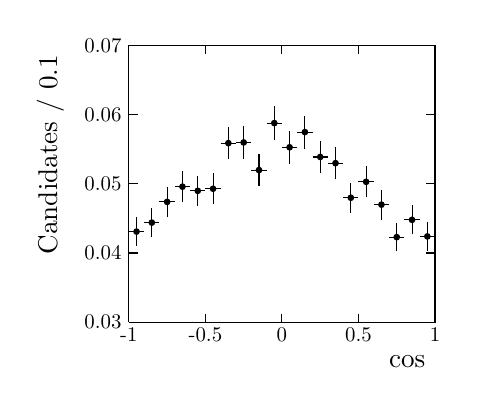
\begin{tikzpicture}
\pgfdeclareplotmark{cross} {
\pgfpathmoveto{\pgfpoint{-0.3\pgfplotmarksize}{\pgfplotmarksize}}
\pgfpathlineto{\pgfpoint{+0.3\pgfplotmarksize}{\pgfplotmarksize}}
\pgfpathlineto{\pgfpoint{+0.3\pgfplotmarksize}{0.3\pgfplotmarksize}}
\pgfpathlineto{\pgfpoint{+1\pgfplotmarksize}{0.3\pgfplotmarksize}}
\pgfpathlineto{\pgfpoint{+1\pgfplotmarksize}{-0.3\pgfplotmarksize}}
\pgfpathlineto{\pgfpoint{+0.3\pgfplotmarksize}{-0.3\pgfplotmarksize}}
\pgfpathlineto{\pgfpoint{+0.3\pgfplotmarksize}{-1.\pgfplotmarksize}}
\pgfpathlineto{\pgfpoint{-0.3\pgfplotmarksize}{-1.\pgfplotmarksize}}
\pgfpathlineto{\pgfpoint{-0.3\pgfplotmarksize}{-0.3\pgfplotmarksize}}
\pgfpathlineto{\pgfpoint{-1.\pgfplotmarksize}{-0.3\pgfplotmarksize}}
\pgfpathlineto{\pgfpoint{-1.\pgfplotmarksize}{0.3\pgfplotmarksize}}
\pgfpathlineto{\pgfpoint{-0.3\pgfplotmarksize}{0.3\pgfplotmarksize}}
\pgfpathclose
\pgfusepathqstroke
}
\pgfdeclareplotmark{cross*} {
\pgfpathmoveto{\pgfpoint{-0.3\pgfplotmarksize}{\pgfplotmarksize}}
\pgfpathlineto{\pgfpoint{+0.3\pgfplotmarksize}{\pgfplotmarksize}}
\pgfpathlineto{\pgfpoint{+0.3\pgfplotmarksize}{0.3\pgfplotmarksize}}
\pgfpathlineto{\pgfpoint{+1\pgfplotmarksize}{0.3\pgfplotmarksize}}
\pgfpathlineto{\pgfpoint{+1\pgfplotmarksize}{-0.3\pgfplotmarksize}}
\pgfpathlineto{\pgfpoint{+0.3\pgfplotmarksize}{-0.3\pgfplotmarksize}}
\pgfpathlineto{\pgfpoint{+0.3\pgfplotmarksize}{-1.\pgfplotmarksize}}
\pgfpathlineto{\pgfpoint{-0.3\pgfplotmarksize}{-1.\pgfplotmarksize}}
\pgfpathlineto{\pgfpoint{-0.3\pgfplotmarksize}{-0.3\pgfplotmarksize}}
\pgfpathlineto{\pgfpoint{-1.\pgfplotmarksize}{-0.3\pgfplotmarksize}}
\pgfpathlineto{\pgfpoint{-1.\pgfplotmarksize}{0.3\pgfplotmarksize}}
\pgfpathlineto{\pgfpoint{-0.3\pgfplotmarksize}{0.3\pgfplotmarksize}}
\pgfpathclose
\pgfusepathqfillstroke
}
\pgfdeclareplotmark{newstar} {
\pgfpathmoveto{\pgfqpoint{0pt}{\pgfplotmarksize}}
\pgfpathlineto{\pgfqpointpolar{44}{0.5\pgfplotmarksize}}
\pgfpathlineto{\pgfqpointpolar{18}{\pgfplotmarksize}}
\pgfpathlineto{\pgfqpointpolar{-20}{0.5\pgfplotmarksize}}
\pgfpathlineto{\pgfqpointpolar{-54}{\pgfplotmarksize}}
\pgfpathlineto{\pgfqpointpolar{-90}{0.5\pgfplotmarksize}}
\pgfpathlineto{\pgfqpointpolar{234}{\pgfplotmarksize}}
\pgfpathlineto{\pgfqpointpolar{198}{0.5\pgfplotmarksize}}
\pgfpathlineto{\pgfqpointpolar{162}{\pgfplotmarksize}}
\pgfpathlineto{\pgfqpointpolar{134}{0.5\pgfplotmarksize}}
\pgfpathclose
\pgfusepathqstroke
}
\pgfdeclareplotmark{newstar*} {
\pgfpathmoveto{\pgfqpoint{0pt}{\pgfplotmarksize}}
\pgfpathlineto{\pgfqpointpolar{44}{0.5\pgfplotmarksize}}
\pgfpathlineto{\pgfqpointpolar{18}{\pgfplotmarksize}}
\pgfpathlineto{\pgfqpointpolar{-20}{0.5\pgfplotmarksize}}
\pgfpathlineto{\pgfqpointpolar{-54}{\pgfplotmarksize}}
\pgfpathlineto{\pgfqpointpolar{-90}{0.5\pgfplotmarksize}}
\pgfpathlineto{\pgfqpointpolar{234}{\pgfplotmarksize}}
\pgfpathlineto{\pgfqpointpolar{198}{0.5\pgfplotmarksize}}
\pgfpathlineto{\pgfqpointpolar{162}{\pgfplotmarksize}}
\pgfpathlineto{\pgfqpointpolar{134}{0.5\pgfplotmarksize}}
\pgfpathclose
\pgfusepathqfillstroke
}
\definecolor{c}{rgb}{1,1,1};
\draw [color=c, fill=c] (0.1,4.72095) rectangle (4.9,9.16419);
\draw [color=c, fill=c] (0.772,5.43186) rectangle (4.66,8.94203);
\definecolor{c}{rgb}{0,0,0};
\draw [c] (0.772,5.43186) -- (0.772,8.94203) -- (4.66,8.94203) -- (4.66,5.43186) -- (0.772,5.43186);
\draw [c,line width=0.4] (0.8692,6.39926) -- (0.8692,6.58144);
\draw [c,line width=0.4] (0.8692,6.58144) -- (0.8692,6.76363);
\draw [c,line width=0.4] (0.772,6.58144) -- (0.8692,6.58144);
\draw [c,line width=0.4] (0.8692,6.58144) -- (0.9664,6.58144);
\foreach \P in {(0.8692,6.58144)}{\draw[mark options={color=c,fill=c},mark size=1.201201pt,mark=*,mark size=1pt] plot coordinates {\P};}
\draw [c,line width=0.4] (1.0636,6.51061) -- (1.0636,6.69552);
\draw [c,line width=0.4] (1.0636,6.69552) -- (1.0636,6.88043);
\draw [c,line width=0.4] (0.9664,6.69552) -- (1.0636,6.69552);
\draw [c,line width=0.4] (1.0636,6.69552) -- (1.1608,6.69552);
\foreach \P in {(1.0636,6.69552)}{\draw[mark options={color=c,fill=c},mark size=1.201201pt,mark=*,mark size=1pt] plot coordinates {\P};}
\draw [c,line width=0.4] (1.258,6.76773) -- (1.258,6.95879);
\draw [c,line width=0.4] (1.258,6.95879) -- (1.258,7.14984);
\draw [c,line width=0.4] (1.1608,6.95879) -- (1.258,6.95879);
\draw [c,line width=0.4] (1.258,6.95879) -- (1.3552,6.95879);
\foreach \P in {(1.258,6.95879)}{\draw[mark options={color=c,fill=c},mark size=1.201201pt,mark=*,mark size=1pt] plot coordinates {\P};}
\draw [c,line width=0.4] (1.4524,6.95641) -- (1.4524,7.15184);
\draw [c,line width=0.4] (1.4524,7.15184) -- (1.4524,7.34728);
\draw [c,line width=0.4] (1.3552,7.15184) -- (1.4524,7.15184);
\draw [c,line width=0.4] (1.4524,7.15184) -- (1.5496,7.15184);
\foreach \P in {(1.4524,7.15184)}{\draw[mark options={color=c,fill=c},mark size=1.201201pt,mark=*,mark size=1pt] plot coordinates {\P};}
\draw [c,line width=0.4] (1.6468,6.90494) -- (1.6468,7.09919);
\draw [c,line width=0.4] (1.6468,7.09919) -- (1.6468,7.29344);
\draw [c,line width=0.4] (1.5496,7.09919) -- (1.6468,7.09919);
\draw [c,line width=0.4] (1.6468,7.09919) -- (1.744,7.09919);
\foreach \P in {(1.6468,7.09919)}{\draw[mark options={color=c,fill=c},mark size=1.201201pt,mark=*,mark size=1pt] plot coordinates {\P};}
\draw [c,line width=0.4] (1.8412,6.93067) -- (1.8412,7.12552);
\draw [c,line width=0.4] (1.8412,7.12552) -- (1.8412,7.32036);
\draw [c,line width=0.4] (1.744,7.12552) -- (1.8412,7.12552);
\draw [c,line width=0.4] (1.8412,7.12552) -- (1.9384,7.12552);
\foreach \P in {(1.8412,7.12552)}{\draw[mark options={color=c,fill=c},mark size=1.201201pt,mark=*,mark size=1pt] plot coordinates {\P};}
\draw [c,line width=0.4] (2.0356,7.49722) -- (2.0356,7.70469);
\draw [c,line width=0.4] (2.0356,7.70469) -- (2.0356,7.91217);
\draw [c,line width=0.4] (1.9384,7.70469) -- (2.0356,7.70469);
\draw [c,line width=0.4] (2.0356,7.70469) -- (2.1328,7.70469);
\foreach \P in {(2.0356,7.70469)}{\draw[mark options={color=c,fill=c},mark size=1.201201pt,mark=*,mark size=1pt] plot coordinates {\P};}
\draw [c,line width=0.4] (2.23,7.50581) -- (2.23,7.71347);
\draw [c,line width=0.4] (2.23,7.71347) -- (2.23,7.92113);
\draw [c,line width=0.4] (2.1328,7.71347) -- (2.23,7.71347);
\draw [c,line width=0.4] (2.23,7.71347) -- (2.3272,7.71347);
\foreach \P in {(2.23,7.71347)}{\draw[mark options={color=c,fill=c},mark size=1.201201pt,mark=*,mark size=1pt] plot coordinates {\P};}
\draw [c,line width=0.4] (2.4244,7.16234) -- (2.4244,7.36245);
\draw [c,line width=0.4] (2.4244,7.36245) -- (2.4244,7.56256);
\draw [c,line width=0.4] (2.3272,7.36245) -- (2.4244,7.36245);
\draw [c,line width=0.4] (2.4244,7.36245) -- (2.5216,7.36245);
\foreach \P in {(2.4244,7.36245)}{\draw[mark options={color=c,fill=c},mark size=1.201201pt,mark=*,mark size=1pt] plot coordinates {\P};}
\draw [c,line width=0.4] (2.6188,7.74639) -- (2.6188,7.95918);
\draw [c,line width=0.4] (2.6188,7.95918) -- (2.6188,8.17197);
\draw [c,line width=0.4] (2.5216,7.95918) -- (2.6188,7.95918);
\draw [c,line width=0.4] (2.6188,7.95918) -- (2.716,7.95918);
\foreach \P in {(2.6188,7.95918)}{\draw[mark options={color=c,fill=c},mark size=1.201201pt,mark=*,mark size=1pt] plot coordinates {\P};}
\draw [c,line width=0.4] (2.8132,7.44568) -- (2.8132,7.65204);
\draw [c,line width=0.4] (2.8132,7.65204) -- (2.8132,7.8584);
\draw [c,line width=0.4] (2.716,7.65204) -- (2.8132,7.65204);
\draw [c,line width=0.4] (2.8132,7.65204) -- (2.9104,7.65204);
\foreach \P in {(2.8132,7.65204)}{\draw[mark options={color=c,fill=c},mark size=1.201201pt,mark=*,mark size=1pt] plot coordinates {\P};}
\draw [c,line width=0.4] (3.0076,7.63467) -- (3.0076,7.8451);
\draw [c,line width=0.4] (3.0076,7.8451) -- (3.0076,8.05553);
\draw [c,line width=0.4] (2.9104,7.8451) -- (3.0076,7.8451);
\draw [c,line width=0.4] (3.0076,7.8451) -- (3.1048,7.8451);
\foreach \P in {(3.0076,7.8451)}{\draw[mark options={color=c,fill=c},mark size=1.201201pt,mark=*,mark size=1pt] plot coordinates {\P};}
\draw [c,line width=0.4] (3.202,7.32545) -- (3.202,7.52919);
\draw [c,line width=0.4] (3.202,7.52919) -- (3.202,7.73292);
\draw [c,line width=0.4] (3.1048,7.52919) -- (3.202,7.52919);
\draw [c,line width=0.4] (3.202,7.52919) -- (3.2992,7.52919);
\foreach \P in {(3.202,7.52919)}{\draw[mark options={color=c,fill=c},mark size=1.201201pt,mark=*,mark size=1pt] plot coordinates {\P};}
\draw [c,line width=0.4] (3.3964,7.24818) -- (3.3964,7.45021);
\draw [c,line width=0.4] (3.3964,7.45021) -- (3.3964,7.65223);
\draw [c,line width=0.4] (3.2992,7.45021) -- (3.3964,7.45021);
\draw [c,line width=0.4] (3.3964,7.45021) -- (3.4936,7.45021);
\foreach \P in {(3.3964,7.45021)}{\draw[mark options={color=c,fill=c},mark size=1.201201pt,mark=*,mark size=1pt] plot coordinates {\P};}
\draw [c,line width=0.4] (3.5908,6.81918) -- (3.5908,7.01144);
\draw [c,line width=0.4] (3.5908,7.01144) -- (3.5908,7.2037);
\draw [c,line width=0.4] (3.4936,7.01144) -- (3.5908,7.01144);
\draw [c,line width=0.4] (3.5908,7.01144) -- (3.688,7.01144);
\foreach \P in {(3.5908,7.01144)}{\draw[mark options={color=c,fill=c},mark size=1.201201pt,mark=*,mark size=1pt] plot coordinates {\P};}
\draw [c,line width=0.4] (3.7852,7.01646) -- (3.7852,7.21327);
\draw [c,line width=0.4] (3.7852,7.21327) -- (3.7852,7.41008);
\draw [c,line width=0.4] (3.688,7.21327) -- (3.7852,7.21327);
\draw [c,line width=0.4] (3.7852,7.21327) -- (3.8824,7.21327);
\foreach \P in {(3.7852,7.21327)}{\draw[mark options={color=c,fill=c},mark size=1.201201pt,mark=*,mark size=1pt] plot coordinates {\P};}
\draw [c,line width=0.4] (3.9796,6.73344) -- (3.9796,6.92368);
\draw [c,line width=0.4] (3.9796,6.92368) -- (3.9796,7.11393);
\draw [c,line width=0.4] (3.8824,6.92368) -- (3.9796,6.92368);
\draw [c,line width=0.4] (3.9796,6.92368) -- (4.0768,6.92368);
\foreach \P in {(3.9796,6.92368)}{\draw[mark options={color=c,fill=c},mark size=1.201201pt,mark=*,mark size=1pt] plot coordinates {\P};}
\draw [c,line width=0.4] (4.174,6.33076) -- (4.174,6.51124);
\draw [c,line width=0.4] (4.174,6.51124) -- (4.174,6.69172);
\draw [c,line width=0.4] (4.0768,6.51124) -- (4.174,6.51124);
\draw [c,line width=0.4] (4.174,6.51124) -- (4.2712,6.51124);
\foreach \P in {(4.174,6.51124)}{\draw[mark options={color=c,fill=c},mark size=1.201201pt,mark=*,mark size=1pt] plot coordinates {\P};}
\draw [c,line width=0.4] (4.3684,6.54488) -- (4.3684,6.73062);
\draw [c,line width=0.4] (4.3684,6.73062) -- (4.3684,6.91637);
\draw [c,line width=0.4] (4.2712,6.73062) -- (4.3684,6.73062);
\draw [c,line width=0.4] (4.3684,6.73062) -- (4.4656,6.73062);
\foreach \P in {(4.3684,6.73062)}{\draw[mark options={color=c,fill=c},mark size=1.201201pt,mark=*,mark size=1pt] plot coordinates {\P};}
\draw [c,line width=0.4] (4.5628,6.33932) -- (4.5628,6.52002);
\draw [c,line width=0.4] (4.5628,6.52002) -- (4.5628,6.70071);
\draw [c,line width=0.4] (4.4656,6.52002) -- (4.5628,6.52002);
\draw [c,line width=0.4] (4.5628,6.52002) -- (4.66,6.52002);
\foreach \P in {(4.5628,6.52002)}{\draw[mark options={color=c,fill=c},mark size=1.201201pt,mark=*,mark size=1pt] plot coordinates {\P};}
\draw [c,line width=0.4] (0.772,5.43186) -- (4.66,5.43186);
\draw [anchor= east] (4.66,4.93422) node[scale=0.979298, rotate=0]{$\cos\thetamu$};
\draw [c,line width=0.4] (0.772,5.53984) -- (0.772,5.43186);
\draw [c,line width=0.4] (1.744,5.53984) -- (1.744,5.43186);
\draw [c,line width=0.4] (2.716,5.53984) -- (2.716,5.43186);
\draw [c,line width=0.4] (3.688,5.53984) -- (3.688,5.43186);
\draw [c,line width=0.4] (4.66,5.53984) -- (4.66,5.43186);
\draw [anchor=base] (0.772,5.19193) node[scale=0.753306, rotate=0]{-1};
\draw [anchor=base] (1.744,5.19193) node[scale=0.753306, rotate=0]{-0.5};
\draw [anchor=base] (2.716,5.19193) node[scale=0.753306, rotate=0]{0};
\draw [anchor=base] (3.688,5.19193) node[scale=0.753306, rotate=0]{0.5};
\draw [anchor=base] (4.66,5.19193) node[scale=0.753306, rotate=0]{1};
\draw [c,line width=0.4] (0.772,8.94203) -- (4.66,8.94203);
\draw [c,line width=0.4] (0.772,8.83406) -- (0.772,8.94203);
\draw [c,line width=0.4] (1.744,8.83406) -- (1.744,8.94203);
\draw [c,line width=0.4] (2.716,8.83406) -- (2.716,8.94203);
\draw [c,line width=0.4] (3.688,8.83406) -- (3.688,8.94203);
\draw [c,line width=0.4] (4.66,8.83406) -- (4.66,8.94203);
\draw [c,line width=0.4] (0.772,5.43186) -- (0.772,8.94203);
\draw [anchor= east] (-0.2264,8.94203) node[scale=0.979298, rotate=90]{Candidates / 0.1};
\draw [c,line width=0.4] (0.88576,5.43186) -- (0.772,5.43186);
\draw [c,line width=0.4] (0.88576,6.30941) -- (0.772,6.30941);
\draw [c,line width=0.4] (0.88576,7.18695) -- (0.772,7.18695);
\draw [c,line width=0.4] (0.88576,8.06449) -- (0.772,8.06449);
\draw [c,line width=0.4] (0.88576,8.94203) -- (0.772,8.94203);
\draw [anchor= east] (0.772,5.43186) node[scale=0.753306, rotate=0]{0.03};
\draw [anchor= east] (0.772,6.30941) node[scale=0.753306, rotate=0]{0.04};
\draw [anchor= east] (0.772,7.18695) node[scale=0.753306, rotate=0]{0.05};
\draw [anchor= east] (0.772,8.06449) node[scale=0.753306, rotate=0]{0.06};
\draw [anchor= east] (0.772,8.94203) node[scale=0.753306, rotate=0]{0.07};
\draw [c,line width=0.4] (4.66,5.43186) -- (4.66,8.94203);
\draw [c,line width=0.4] (4.54624,5.43186) -- (4.66,5.43186);
\draw [c,line width=0.4] (4.54624,6.30941) -- (4.66,6.30941);
\draw [c,line width=0.4] (4.54624,7.18695) -- (4.66,7.18695);
\draw [c,line width=0.4] (4.54624,8.06449) -- (4.66,8.06449);
\draw [c,line width=0.4] (4.54624,8.94203) -- (4.66,8.94203);
\end{tikzpicture}
